% =====================================================================
%  DRAFT for the course project. Formatted to approximate the ICASSP
%  two-column style so it compiles with a stock TeX Live installation.
%
%  TO SUBMIT WITH THE OFFICIAL ICASSP TEMPLATE:
%    1. Download the ICASSP Paper Kit (spconf.sty + template).
%    2. Replace the preamble block below (down to \begin{document}) with:
%         \documentclass{article}
%         \usepackage{spconf,amsmath,graphicx,booktabs}
%       and use \title{...}, \name{...}, \address{...}, \maketitle.
%    3. The body, tables, figures and references below transfer unchanged.
% =====================================================================
\documentclass[10pt,twocolumn,letterpaper]{article}
\usepackage[letterpaper,top=0.75in,bottom=1.0in,left=0.75in,right=0.75in,columnsep=0.3in]{geometry}
\usepackage{mathptmx}          % Times-like font (as ICASSP)
\usepackage{graphicx,amsmath,amssymb,booktabs,url}
\usepackage[hidelinks]{hyperref}
\usepackage{caption}
\captionsetup{font=small,labelfont=bf}
\pagestyle{empty}

\title{\textbf{\large What Matters in Frozen Self-Supervised Representations\\
for Low-Resource ASR: A Controlled Study of Layer and Decoder Choice}}
\author{
Group members: \emph{Name 1 (ID)}, \emph{Name 2 (ID)}, \emph{Name 3 (ID)}\\
\small Course Project --- Self-Supervised Speech Representation Learning
}
\date{}

\begin{document}
\maketitle
\thispagestyle{empty}

\begin{abstract}
Self-supervised speech models such as wav2vec~2.0 are widely used as
\emph{frozen} feature extractors for low-resource ASR, yet several practical
choices remain under-documented: which encoder layer to tap, how complex the
downstream decoder should be, and how much labelled data is needed. We present
a controlled study on LibriSpeech that isolates these three axes under a single
fixed-budget setup with a frozen wav2vec~2.0 encoder and a character-level CTC
head. We find that (i)~the representation layer is the single largest lever---a
middle layer (9) reduces WER from $0.86$ (final layer) to $0.30$---because the
pretraining-only encoder's top layers specialise to the pretext task;
(ii)~a simple non-linear per-frame head is sufficient: a two-layer MLP matches
or beats a Transformer decoder with $4.3\times$ the parameters, indicating that
cross-frame modelling is largely redundant with the encoder's own context; and
(iii)~inference latency is dominated by the encoder forward pass, so decoder
size (a $77\times$ range) barely changes RTF. Data scaling exhibits clear
diminishing returns, suggesting that \emph{adapting} the representation rather
than adding data is the more promising direction.
\end{abstract}

\noindent\textbf{Index Terms}---self-supervised learning, wav2vec 2.0,
low-resource ASR, CTC, representation probing.

\section{Introduction}
Self-supervised learning (SSL) models---wav2vec~2.0~\cite{w2v2},
HuBERT~\cite{hubert}, WavLM~\cite{wavlm}---are pretrained on large amounts of
unlabelled speech and yield general-purpose representations that transfer well
to downstream tasks. A dominant recipe for low-resource ASR is to \emph{freeze}
the SSL encoder and train only a lightweight downstream head on top, a form of
representation probing that avoids overfitting the millions of encoder
parameters on scarce labelled data.

While this recipe is common, three design decisions are usually made by
convention rather than measurement: (1)~\emph{which} of the encoder's many
Transformer layers to use, (2)~how \emph{complex} the downstream decoder should
be, and (3)~how much labelled data is actually required. These are rarely
answered together under one controlled setting. In this paper we hold a single
baseline system fixed and vary exactly one factor at a time, on LibriSpeech,
with a frozen wav2vec~2.0 encoder and a character-level CTC head.

Our contributions are: (i)~a controlled ablation across representation layer,
decoder structure and data size that ranks their importance for frozen-SSL
low-resource ASR; (ii)~the observation that a simple non-linear per-frame head
suffices, while added cross-frame capacity is redundant with the encoder's own
contextualisation; and (iii)~the finding that, under a frozen encoder,
inference latency is set by the encoder and is essentially independent of
decoder size, so accuracy and decoder complexity are decoupled from speed.

\section{Method}
\subsection{Frozen SSL encoder}
We use \texttt{wav2vec2-base}~\cite{w2v2}, kept frozen throughout. A
seven-layer convolutional feature encoder downsamples the $16$\,kHz waveform by
a factor of $320$, producing one $512$-d frame every $20$\,ms ($50$ frames/s).
A $12$-layer Transformer then produces contextual hidden states. We expose the
hidden states of a chosen layer $l$ and treat them as fixed features.

\subsection{Representation and CTC head}
The selected hidden states $C\in\mathbb{R}^{T\times768}$ are passed to a
downstream decoder that emits, for every frame, a distribution over a
$30$-token character vocabulary (blank, unknown, space, apostrophe and the
$26$ letters). The model is trained with the CTC objective~\cite{ctc}, which
marginalises over all frame-to-character alignments and requires no
frame-level supervision. At inference we use greedy decoding: per-frame
$\arg\max$, followed by collapsing repeats and removing blanks. The full
pipeline is shown in Fig.~\ref{fig:system}.

\begin{figure}[t]
\centering
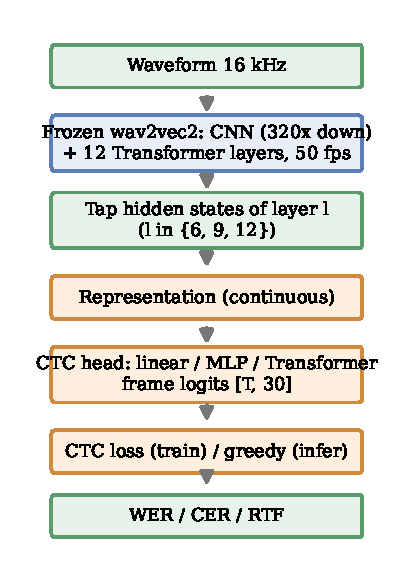
\includegraphics[width=0.80\linewidth]{figures/fig_system.pdf}
\caption{System pipeline. The SSL encoder (blue) is frozen; only the
representation and CTC head (orange) are trained. Our three ablation axes are
the tapped layer $l$, the decoder structure, and the amount of training data.}
\label{fig:system}
\end{figure}

\subsection{Decoder variants}
We compare three heads that all preserve the time axis (so CTC alignment is
unaffected): a \textbf{linear} head (a single projection; a pure linear probe),
an \textbf{MLP} head (LayerNorm, a hidden layer with GELU, then a projection;
non-linear but still per-frame), and a \textbf{Transformer} head (an input
projection, sinusoidal positional encoding and two self-attention layers; the
only variant that mixes information across frames).

\section{Experimental Setup}
Experiments use LibriSpeech (clean)~\cite{librispeech} in streaming mode, with
$3600$ training and $500$ validation utterances at $16$\,kHz for the baseline.
All systems are trained under a single \emph{fixed budget}: $10$ epochs, batch
size $8$, learning rate $10^{-3}$ with a cosine schedule and early stopping,
and a single random seed. We therefore report a fixed-budget comparison rather
than converged numbers; this is revisited in Section~\ref{sec:disc}. Unless
noted, the baseline is \{\,wav2vec2-base frozen, layer~9, MLP head,
$3600$ utterances\,\}, and each study perturbs exactly one factor. We report
Word and Character Error Rate (WER/CER), the Real-Time Factor (RTF), and the
substitution/deletion/insertion counts for error analysis.

\section{Results and Analysis}
\subsection{Which layer? (Representation layer)}
Table~\ref{tab:layer} and Fig.~\ref{fig:layer} vary the tapped layer with the
head, data and budget fixed. A middle layer (9) is clearly best, while the
final layer (12) is dramatically worst. This reproduces the well-known
acoustic$\rightarrow$linguistic$\rightarrow$pretext trajectory of SSL
representations~\cite{pasad}: because \texttt{wav2vec2-base} is
pretrained-only (never fine-tuned for ASR), its top layers specialise back to
the contrastive/quantisation pretext objective and lose directly usable content
information. Simply changing the tapped layer lowers WER from $0.86$ to $0.30$
(a $\sim$66\% relative reduction) at \emph{zero} additional parameters or
training---the largest single lever in this study.

\begin{table}[t]
\centering
\caption{Layer ablation (MLP head, $3600$ utterances, $10$ epochs).
S/D/I = substitutions/deletions/insertions.}
\label{tab:layer}
\small
\begin{tabular}{cccccc}
\toprule
Layer & WER & CER & Val.\ loss & S/D/I \\
\midrule
6           & 0.4138 & 0.1186 & 0.4604 & 3334/301/300 \\
\textbf{9}  & \textbf{0.2954} & \textbf{0.0768} & \textbf{0.3088} & 2459/238/112 \\
12 (final)  & 0.8596 & 0.3426 & 1.1925 & 6150/1837/188 \\
\bottomrule
\end{tabular}
\end{table}

\begin{figure}[t]
\centering
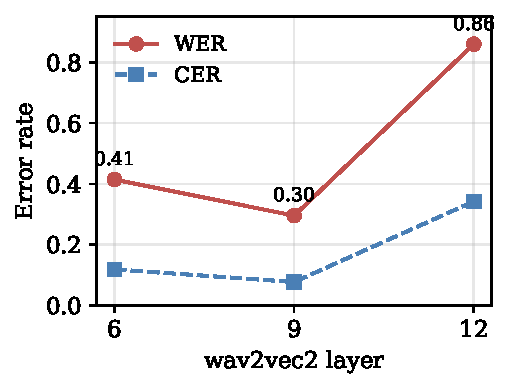
\includegraphics[width=0.82\linewidth]{figures/fig_layer.pdf}
\caption{WER and CER as a function of the tapped wav2vec2 layer. The middle
layer is best; the final layer collapses.}
\label{fig:layer}
\end{figure}

\subsection{How complex a decoder? (Decoder structure)}
Table~\ref{tab:dec} and Fig.~\ref{fig:dec} vary the head at the best layer~(9).
Two effects stand out. First, \emph{non-linearity is the main lever}: moving
from the linear probe to the MLP cuts WER from $0.60$ to $0.30$
($\sim$51\% relative), showing that the layer-9 features are not fully linearly
separable but a single non-linear per-frame mapping recovers most of the gap.
Second, \emph{cross-frame modelling does not help}: the Transformer head
($1.78$M parameters) is slightly worse than the MLP ($0.41$M). Two factors
explain this: (a)~wav2vec~2.0 is itself a $12$-layer Transformer, so its
layer-9 features are already strongly contextualised and an extra Transformer is
redundant; and (b)~under the fixed $10$-epoch budget the larger head is
under-optimised---its validation loss ($0.3922$) is \emph{higher} than the
MLP's ($0.3088$), which indicates under-fitting rather than over-fitting. We
therefore state only that cross-frame capacity gives no gain \emph{under this
budget}, without claiming it is fundamentally inferior.

Finally, RTF is essentially constant ($0.010$--$0.011$) across a $77\times$
range of decoder parameters. Because the frozen encoder forward pass dominates
computation, decoder complexity is decoupled from inference speed: one can
choose the head on accuracy grounds alone.

\begin{table}[t]
\centering
\caption{Decoder ablation (layer 9, $3600$ utterances, $10$ epochs).}
\label{tab:dec}
\small
\begin{tabular}{lccccc}
\toprule
Decoder & Params & WER & CER & Val.\ loss & RTF \\
\midrule
Linear      & 23{,}070    & 0.6027 & 0.1846 & 0.6456 & 0.0102 \\
\textbf{MLP}& 410{,}654   & \textbf{0.2954} & \textbf{0.0768} & \textbf{0.3088} & 0.0111 \\
Transformer & 1{,}784{,}094 & 0.3163 & 0.0845 & 0.3922 & 0.0104 \\
\bottomrule
\end{tabular}
\end{table}

\begin{figure}[t]
\centering
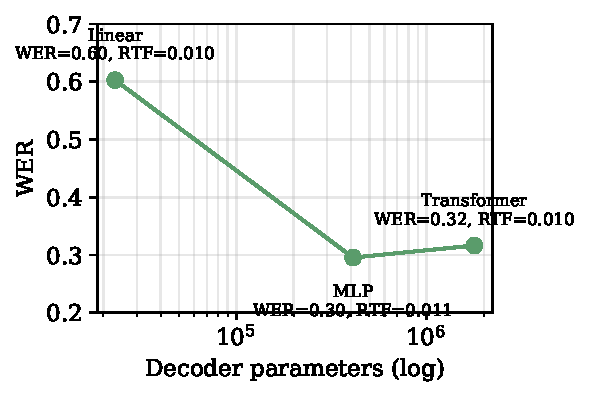
\includegraphics[width=0.82\linewidth]{figures/fig_decoder.pdf}
\caption{WER versus decoder parameters (log scale). A non-linear MLP is best;
the much larger Transformer does not improve accuracy, and RTF is essentially
unchanged.}
\label{fig:dec}
\end{figure}

\subsection{How much data? (Training-set size)}
Table~\ref{tab:data} and Fig.~\ref{fig:data} scale the training set from
$900$ to $7200$ utterances (layer 9, MLP). WER decreases monotonically but with
clear diminishing returns: doubling from $900$ to $1800$ helps substantially
($0.43\rightarrow0.34$), whereas doubling from $3600$ to $7200$ yields only
$0.30\rightarrow0.25$ ($\sim$16\% relative). The flattening curve suggests that
a frozen representation with a lightweight head is approaching a ceiling, and
that further gains are more likely to come from \emph{adapting} the
representation (e.g.\ parameter-efficient fine-tuning~\cite{lora}) than from
additional labelled data.

\begin{table}[t]
\centering
\caption{Training-set size (layer 9, MLP head, $10$ epochs).}
\label{tab:data}
\small
\begin{tabular}{cccccc}
\toprule
Utterances & 900 & 1800 & 3600 & 5400 & 7200 \\
\midrule
WER & 0.4278 & 0.3449 & 0.2954 & 0.2579 & 0.2493 \\
CER & 0.1174 & 0.0911 & 0.0768 & 0.0674 & 0.0634 \\
\bottomrule
\end{tabular}
\end{table}

\begin{figure}[t]
\centering
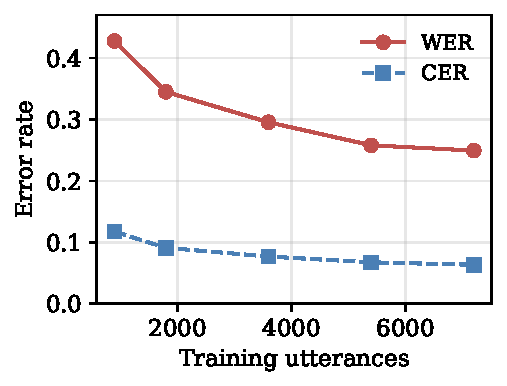
\includegraphics[width=0.82\linewidth]{figures/fig_data.pdf}
\caption{WER and CER versus training-set size. Errors fall with clear
diminishing returns.}
\label{fig:data}
\end{figure}

\subsection{Error analysis}
Across configurations, healthy systems (layer 9, MLP, larger data) are
dominated by \emph{substitutions} with few deletions. In contrast, the two
failing configurations---the final layer and the linear head---show sharply
elevated \emph{deletions} ($1837$ and $828$ respectively, versus $\sim$238 for
the baseline out of $9510$ reference words). This is the signature of a
blank-dominated CTC output collapsing toward empty transcriptions, and it
matches the large CER/WER gap of the final layer (CER $0.34$ but WER $0.86$):
characters are partially correct but almost no whole word is, indicating an
under-optimised or mismatched representation rather than random output.

\subsection{Synthesis}
Anchored at layer~9, the three axes can be ranked by leverage:
\emph{representation layer} $\gg$ \emph{per-frame non-linearity} $>$
\emph{data size} $>$ \emph{cross-frame capacity} ($\approx0$). In short, for
frozen-SSL low-resource ASR, what matters is choosing the right layer and a
simple non-linear head; extra decoder capacity and additional data both give
limited marginal returns.

\section{Discussion and Limitations}
\label{sec:disc}
All results use a fixed $10$-epoch budget and a single seed, so they should be
read as a fixed-budget comparison; larger heads such as the Transformer may be
under-trained (as their higher validation loss suggests), and longer training
or multiple seeds would tighten the close comparisons. As preliminary work
toward discrete units, we also implemented a k-means discretisation path
(continuous features $\rightarrow$ cluster id $\rightarrow$ trainable embedding
$\rightarrow$ CTC) that reports token rate, bitrate and codebook utilisation;
however, under the same tight budget the from-scratch unit embedding did not
train well, so we do not report discrete ASR accuracy as a reliable result and
leave it to future work. Promising directions include parameter-efficient
adaptation of the encoder (e.g.\ LoRA) to break the data ceiling, feature
caching to afford longer training, and cross-model comparison with HuBERT and
WavLM.

\section{Conclusion}
We presented a controlled study of frozen wav2vec~2.0 features for low-resource
CTC ASR. The tapped layer is the dominant factor---a middle layer far
outperforms the pretraining-specialised final layer---while a simple non-linear
per-frame head is sufficient and added cross-frame modelling is redundant with
the encoder's own context. Inference latency is set by the frozen encoder, and
data scaling shows diminishing returns. The practical recommendation is to
spend effort on layer selection and a lightweight non-linear head, and to
reserve compute for adapting the representation rather than enlarging the
decoder or the dataset.

\begin{thebibliography}{9}
\small
\bibitem{w2v2} A.~Baevski, Y.~Zhou, A.~Mohamed, and M.~Auli,
``wav2vec 2.0: A framework for self-supervised learning of speech
representations,'' in \emph{NeurIPS}, 2020.
\bibitem{hubert} W.-N.~Hsu \emph{et al.},
``HuBERT: Self-supervised speech representation learning by masked prediction
of hidden units,'' \emph{IEEE/ACM TASLP}, 2021.
\bibitem{wavlm} S.~Chen \emph{et al.},
``WavLM: Large-scale self-supervised pre-training for full stack speech
processing,'' \emph{IEEE JSTSP}, 2022.
\bibitem{ctc} A.~Graves, S.~Fern\'andez, F.~Gomez, and J.~Schmidhuber,
``Connectionist temporal classification: Labelling unsegmented sequence data
with recurrent neural networks,'' in \emph{ICML}, 2006.
\bibitem{pasad} A.~Pasad, J.-C.~Chou, and K.~Livescu,
``Layer-wise analysis of a self-supervised speech representation model,''
in \emph{IEEE ASRU}, 2021.
\bibitem{librispeech} V.~Panayotov, G.~Chen, D.~Povey, and S.~Khudanpur,
``Librispeech: An ASR corpus based on public domain audio books,''
in \emph{ICASSP}, 2015.
\bibitem{lora} E.~J.~Hu \emph{et al.},
``LoRA: Low-rank adaptation of large language models,'' in \emph{ICLR}, 2022.
\end{thebibliography}

\end{document}
